                                                                                                                      \documentclass[11pt,a4paper]{report}

\usepackage[utf8]{inputenc}
\usepackage[T1]{fontenc}

\pagestyle{empty}

\usepackage{graphicx} % Include figure files
\usepackage{amstext,amsbsy,amssymb}
%\usepackage{times} 

%% Numbered problems
\newcounter{excount}[chapter]
\newenvironment{exercise}[1][]{\addtocounter{excount}{1} \noindent {\bf Problem
    \arabic{excount} \ \ #1}\hspace{2mm}}{\vspace{4mm}}


\title{FYS3120 Classical Mechanics and Electrodynamics\\ 
\vspace{15mm}Problem set 6}


%%%%%%%
\begin{document}
%%%%%%%
\maketitle


%%%%%%%%
\begin{exercise}
This problem is an exercise in using space-time diagrams (Minkowski diagrams) when studying how elementary relativistic effects are represented in different inertial reference frames. 
%The use of Lorentz transformations should therefore be avoided.

A railway carriage is moving in a straight line with constant velocity $v$ relative to the earth. The earth is considered as an inertial reference frame $S$, and in this reference frame the moving carriage has the length $L$. The situation is shown in Fig.~\ref{fig:tog}, where
$A$ and $B$ indicate points on the rear wall and front wall of the carriage, respectively. C is a point in the middle of the carriage.

%%%%%%%%%%
\begin{figure}[h]
\begin{center}
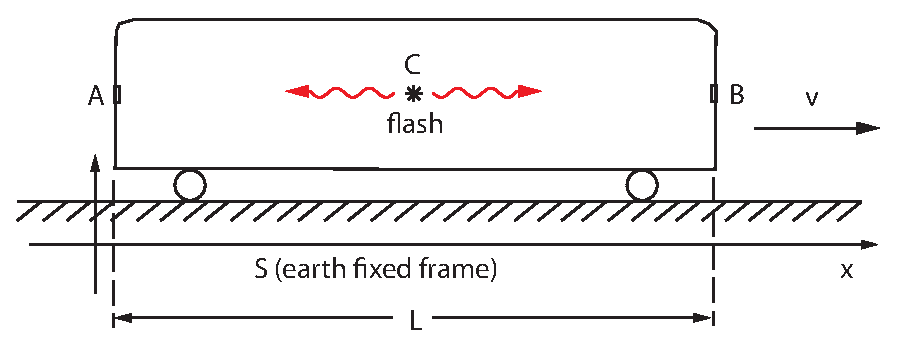
\includegraphics[width=9cm]{Tog.eps}
\end{center}
\caption{Diagram of the railway carriage.}
\label{fig:tog}
\end{figure}
%%%%%%%%%% 

\begin{itemize}
\item[\bf a)] In Fig.~\ref{fig:minkowski} we have drawn the world line (space-time trajectory) for the midpoint C in a two-dimensional Minkowski diagram of reference frame $S$. Draw the world lines for the points A and B in the same diagram and show that the angle $\alpha$ between these lines and the time axis is given by $\tan\alpha=v/c$. (Choose the origin of the coordinate system in $S$ so that $A$ has coordinate $x=0$ at time $t=0$.)

%%%%%%%%%%
\begin{figure}[h]
\begin{center}
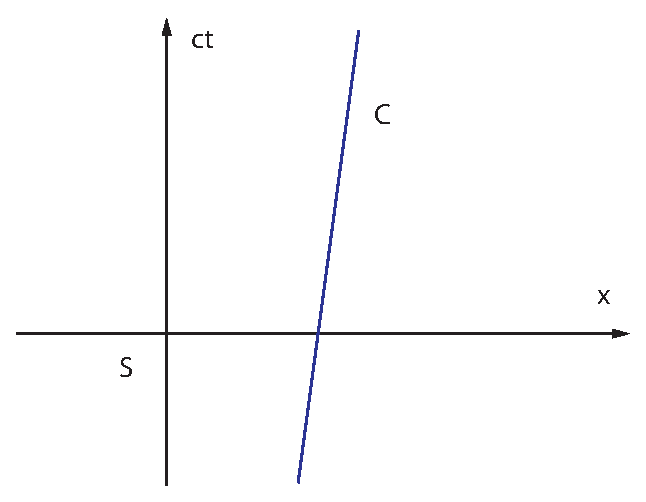
\includegraphics[width=6cm]{C-trajectory.eps}
\end{center}
\caption{Minkowski diagram for reference frame $S$.}
\label{fig:minkowski}
\end{figure}
%%%%%%%%%% 

\begin{figure}[h]
\begin{center}
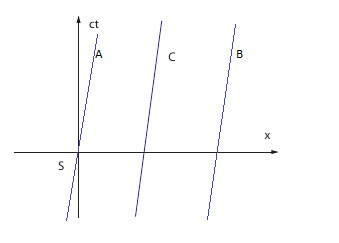
\includegraphics[width=9cm]{draw1.png}
\end{center}
\caption{1.a) Minkowski diagram for reference frame $S$, including world lines for A and B.}
\label{fig:tog}
\end{figure}
\item $ct'$ sin $\alpha = vt$, $ct'$ cos $\alpha = ct$, thus tan$ \alpha =  v/c $
\end{itemize}

At a given time $t_0$ a flash tube is discharged at point C. We will call this event (space-time point)  $E_0$. Some of the light will propagate backwards in the compartment and some will propagate forwards. Let $E_1$ and  $E_2$ be the events where the light signals hit the rear wall and front wall, respectively. Let us assume that the light is reflected from A and B, and that the two reflected light signals meet at a space-time point $E_3$.  


\begin{itemize}
\item[\bf b)] Draw the world lines of the light signals as well as the four events $E_0$, $E_1$, $E_2$ and $E_3$ in the Minkowski diagram of reference frame $S$. 
\begin{figure}[h]
\begin{center}
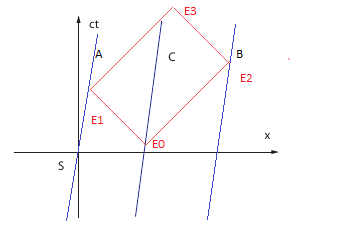
\includegraphics[width=9cm]{draw2.png}
\end{center}
\caption{1.b) Minkowski diagram for reference frame $S$, with events $E_i, i=0,1,2,3$}
\label{fig:tog}
\end{figure}


\item[\bf c)] We introduce the co-moving reference frame $S'$ of the carriage. Explain why $E_1$ and $E_2$ are simultaneous in this reference frame and why $E_0$ and $E_3$ are at the same point in space in S'. Is this consistent with the drawing of point {\bf b)}?

\item $E_1$ and $E_2$ are simultaneous in RF $S'$, as the distance from $C$ to either $A$ or $B$ is the same, and for an observer at rest in $S'$, the points $A$ and $B$ are not moving, thus the light signals will use the same time from $C$ to either $A$ or $B$. With the same logic, $E_3$ will occur at the same point as $E_0$ as the reflected light signals will arrive at the same time at $C$, observed from within $S'$. This is consistent with the drawing made in $b)$, as that drawing shows the events as seen from RF $S$, not $S'$ - although in $S$, $E_3$ does not occur at $C$.

\item[\bf d)] Draw the straight line from from $E_1$ to $E_2$ in the Minkowski diagram of $S$ and show that the angle between the $x$-axis and this line is $\alpha$. 
\item[\bf e)] Show that if a signal should connect the two space-time points $E_1$ and $E_2$ it must have the velocity $c^2/v$, which is greater than $c$ and thus forbidden.
\end{itemize}
\end{exercise}


%%%%%%%%
\begin{exercise}
 A thin rigid rod has rest length $L_0$ (length measured in its rest frame). It moves relative to an inertial reference frame $S'$, so that the midpoint $A$ of the rod has the time dependent coordinates $x_A'=0$, $y_A'=u t'$, $z_A'=0$, with $u$ as the velocity of the rod. In this reference frame the rod is at all times parallel to the $x'$ axis.
 
 
\begin{itemize}

\item[\bf a)] Let $B$ be one of the end points of the rod. What are the time dependent coordinates of this point measured in $S'$?


\item $x_B'=L_0/2, y_B'=ut',z_B'=0$

\item[\bf b)]The inertial frame $S'$ moves with velocity $v$ along the $x$-axis relative to another inertial frame $S$. (The axes of the two frames are parallel.) Find the space coordinates $(x,y,z)$ of the points $A$ and $B$ as functions of the time coordinate $t$  in the reference frame $S$. 
 (Remember that if the time coordinate $t$ in $S$ is fixed, the time coordinates $t'_A$ and $t'_B$ of the points $A$ and $B$ are not the same.)
\item[\bf c)]Show that the the rod is not oriented along the $x$-axis in $S$, by calculating the ratio $\tan\phi=(y_B-y_A)/(x_B-x_A)$. What is  the length of the rod measured in this frame?
\end{itemize}
\end{exercise}
 
 
\end{document}
 

